\section{Discussion}

Looking at the results, the interaction were various depending on the plant. 
Thus, we can extract main interactions that are linked to the plant type. 
Looking at table \ref{tab:results}, people are more inclined to use their hands as tam tam or grasp the \textit{Pachira glabra}. 
However, for the \textit{Dracaena} users prefer to pinch the trunk or leave. 
Participants decided to grasp whether a pack of trunk or leaves when it came to \textit{Dypsis lutescens}.
This is induced by many factors including the leaves shape, the width of the trunk.


It was observed that when the plants were positioned at higher elevations on the table, individuals tended to engage more with the trunk of the plants.

Looking at table \ref{tab:results}, we decided to group interaction. This was done by grouping type of interaction depending on 3 main factors :

\begin{itemize}
    \item The intensity factor : what is the intensity of the interaction (ex : pinch is lighter than grasp)
    \item The spatial factor : what is the interaction displacement.
    \item The duration factor : what is the interaction duration (ex : tam tam is instantaneous).
\end{itemize}

The "Group 1" includes the pinch and grasp interaction. Indeed, looking at the 3 factors we defined, 
the pinch and grasp are high in intensity and long in duration but people stay still in space.
This group of interaction can be defined as \textbf{binary interaction}. The user is either grasping or not.

The "Group 2" includes the slide. The slide interaction is long in time, it moves in space but low in intensity.
This group of interaction can be defined as \textbf{continuous interaction}.


Whereas, the "Group 3" includes the pet and Tam Tam. 
These 2 interactions are really high in intensity, people usually tam tam and pet in different places but those interactions are short in time. 
This group is defined as \textbf{repetitive interaction}. The user is repeating the same action over and over again.


\begin{figure}

    \begin{minipage}{.5\linewidth}
    \centering
    \subfloat[]{
        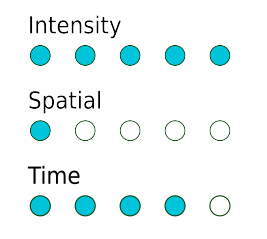
\includegraphics[scale=.4]{Images/group_1_int_dia.png}
        
        \label{fig:interactions:subfig:group1}
        }
    \end{minipage}%
    \begin{minipage}{.5\linewidth}
    \centering
    \subfloat[]{\label{fig:interactions:subfig:group2}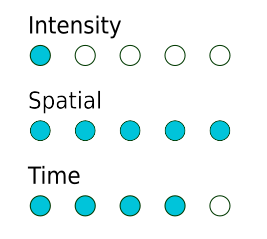
\includegraphics[scale=.4]{Images/group_2_int_dia.png}}
    \end{minipage}\par\medskip
    \centering
    \subfloat[]{\label{fig:interactions:subfig:group3}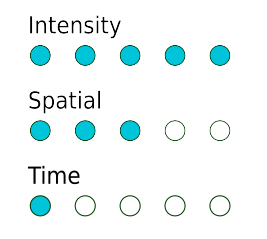
\includegraphics[scale=.4]{Images/group_3_int_dia.png}}
    
    \caption{Figure showing graphically the intensity of the 3 types of factors we defined. (a) Group 1 : pinch and grasp. (b) Group 2 : slide. (c) Group 3 : pet and tam tam.}
    \label{fig:main}
    \end{figure}


The participants we interviewed introduced a bias in the results.
They were all students from the engineering school and thus, they all had a similar background.
Some of them were already familiar with the project.
